\documentclass[11pt,]{article}
\usepackage{lmodern}
\usepackage{amssymb,amsmath}
\usepackage{ifxetex,ifluatex}
\usepackage{fixltx2e} % provides \textsubscript
\ifnum 0\ifxetex 1\fi\ifluatex 1\fi=0 % if pdftex
  \usepackage[T1]{fontenc}
  \usepackage[utf8]{inputenc}
\else % if luatex or xelatex
  \ifxetex
    \usepackage{mathspec}
  \else
    \usepackage{fontspec}
  \fi
  \defaultfontfeatures{Ligatures=TeX,Scale=MatchLowercase}
\fi
% use upquote if available, for straight quotes in verbatim environments
\IfFileExists{upquote.sty}{\usepackage{upquote}}{}
% use microtype if available
\IfFileExists{microtype.sty}{%
\usepackage{microtype}
\UseMicrotypeSet[protrusion]{basicmath} % disable protrusion for tt fonts
}{}
\usepackage[margin=1in]{geometry}
\usepackage{hyperref}
\hypersetup{unicode=true,
            pdftitle={Does oil volatility scale with increasing price?},
            pdfauthor={James Hamski (james.hamski@spsmail.cuny.edu)},
            pdfborder={0 0 0},
            breaklinks=true}
\urlstyle{same}  % don't use monospace font for urls
\usepackage{longtable,booktabs}
\usepackage{graphicx,grffile}
\makeatletter
\def\maxwidth{\ifdim\Gin@nat@width>\linewidth\linewidth\else\Gin@nat@width\fi}
\def\maxheight{\ifdim\Gin@nat@height>\textheight\textheight\else\Gin@nat@height\fi}
\makeatother
% Scale images if necessary, so that they will not overflow the page
% margins by default, and it is still possible to overwrite the defaults
% using explicit options in \includegraphics[width, height, ...]{}
\setkeys{Gin}{width=\maxwidth,height=\maxheight,keepaspectratio}
\IfFileExists{parskip.sty}{%
\usepackage{parskip}
}{% else
\setlength{\parindent}{0pt}
\setlength{\parskip}{6pt plus 2pt minus 1pt}
}
\setlength{\emergencystretch}{3em}  % prevent overfull lines
\providecommand{\tightlist}{%
  \setlength{\itemsep}{0pt}\setlength{\parskip}{0pt}}
\setcounter{secnumdepth}{5}
% Redefines (sub)paragraphs to behave more like sections
\ifx\paragraph\undefined\else
\let\oldparagraph\paragraph
\renewcommand{\paragraph}[1]{\oldparagraph{#1}\mbox{}}
\fi
\ifx\subparagraph\undefined\else
\let\oldsubparagraph\subparagraph
\renewcommand{\subparagraph}[1]{\oldsubparagraph{#1}\mbox{}}
\fi

%%% Use protect on footnotes to avoid problems with footnotes in titles
\let\rmarkdownfootnote\footnote%
\def\footnote{\protect\rmarkdownfootnote}

%%% Change title format to be more compact
\usepackage{titling}

% Create subtitle command for use in maketitle
\newcommand{\subtitle}[1]{
  \posttitle{
    \begin{center}\large#1\end{center}
    }
}

\setlength{\droptitle}{-2em}
  \title{Does oil volatility scale with increasing price?}
  \pretitle{\vspace{\droptitle}\centering\huge}
  \posttitle{\par}
  \author{James Hamski
(\href{mailto:james.hamski@spsmail.cuny.edu}{\nolinkurl{james.hamski@spsmail.cuny.edu}})}
  \preauthor{\centering\large\emph}
  \postauthor{\par}
  \predate{\centering\large\emph}
  \postdate{\par}
  \date{5/19/2017}


\begin{document}
\maketitle

\section{Introduction}\label{introduction}

In a commodity trading market the price level is expected to be tied to
the system dynamics, namely supply, demand, and delivery of the
commodity being traded. Volatility, the variation in price over time,
reflects uncertainty in the balance of these system factors. This
research paper aims to answer a simply posed question: ``does oil price
volatility scale with price?''; i.e., can we expect to observe larger
price swings when the price is near \$100 per barrel vs \$20 per barrel?

If oil price volatility reflects uncertainty about supply and demand
dynamics, it isn't immediately clear whether we should expect volatility
to depend on price level. Higher oil prices are associated with
``tightness'' in the supply market, meaning there is little excess
capacity to increase production, therefore we may expect swings higher
but some base price support that results in lower measured volatility.
Likewise, low prices may suggest excess capacity that can buffer shocks
to the oil delivery system, dampening volatility. Despite these ``just
so'' arguments, a multitude of factors such as storage dynamics, supply
chain distruptions, the ability of producers to increase production to
bring more oil to market or shut in production capacity in response to
prices (``rebalancing''), and market speculation complicate this picture
and suggest it must be studied empirically.

If it is found that oil price volatility is dependent on price level,
the relationship may follow a scaling formula. For instance, if we can
expect volatility of \$1/barrel when oil is at \$20/barrel, can we
expect volatility of \$5/barrel at \$100/barrel price levels via a
simple linear scaling rule? Three methods are presented in this research
paper to answer this question: (1) regression modeling of price and
volatility, (2) viewing volatility within oil price regimes, and (3)
using multivariate Generalized Autoregressive Conditional
Heteroskedasticity (GARCH) modeling.

Note that in this research paper \emph{oil price} is used to
specifically mean spot-traded crude oil. This represents only one
component of the oil markets, and most of the actual oil price is
determined by futures and long term delivery contracts (need cite). This
research paper is concerned with understanding the energy system using
pricing information. In this way, it differs from much of the published
research in that it is not concerned with forecasting prices or
volatility. Nor is it addressing exogeneous system elements such as
equity markets or interest rates, though the literature shows that the
crude oil market and larger economic indicators are intertwined (add
cite). Instead, it contributes to our understanding of the system
dynamics of an essential energy commodity.

\section{Exploratory Data Analysis}\label{exploratory-data-analysis}

\subsection{Data Source}\label{data-source}

The data source is the West Texas Intermediate (WTI) nominal (i.e.~not
inflation adjusted) daily spot price record from the U.S. Energy
Information Administration. The WTI series was filtered to the date
range January 2, 1986 through December 30, 2016.

\begin{longtable}[]{@{}lll@{}}
\caption{Oil price series date and price ranges.}\tabularnewline
\toprule
& Date Range & Price Range\tabularnewline
\midrule
\endfirsthead
\toprule
& Date Range & Price Range\tabularnewline
\midrule
\endhead
& Min. :1986-01-03 & Min. : 10.25\tabularnewline
& 1st Qu.:1993-09-01 & 1st Qu.: 19.38\tabularnewline
& Median :2001-06-11 & Median : 28.01\tabularnewline
& Mean :2001-06-19 & Mean : 42.87\tabularnewline
& 3rd Qu.:2009-03-31 & 3rd Qu.: 63.47\tabularnewline
& Max. :2016-12-30 & Max. :145.31\tabularnewline
\bottomrule
\end{longtable}

\subsection{Returns and Volatility}\label{returns-and-volatility}

In this research paper, volatility is characterized two ways: (1) 5-day
historic volatility and (2) 30-day historic volatility. In addition, the
relationship between the returns themselves and price level is
investigated. Daily returns were calculated as:
\[R_t = \frac{P_t-P_{t-1}}{P_{t-1}}\] In some sections, their absolute
values are used. A seen in Figure 1, most of the series from 1986
through 2004 contains prices between \$10/barrel and \$40/barrel. This
results in a price series with left skew and a long right tail (Figure
2). The return series indicates heteroscedasticity. These distribution
characteristics are common in financial time series.

\begin{figure}[htbp]
\centering
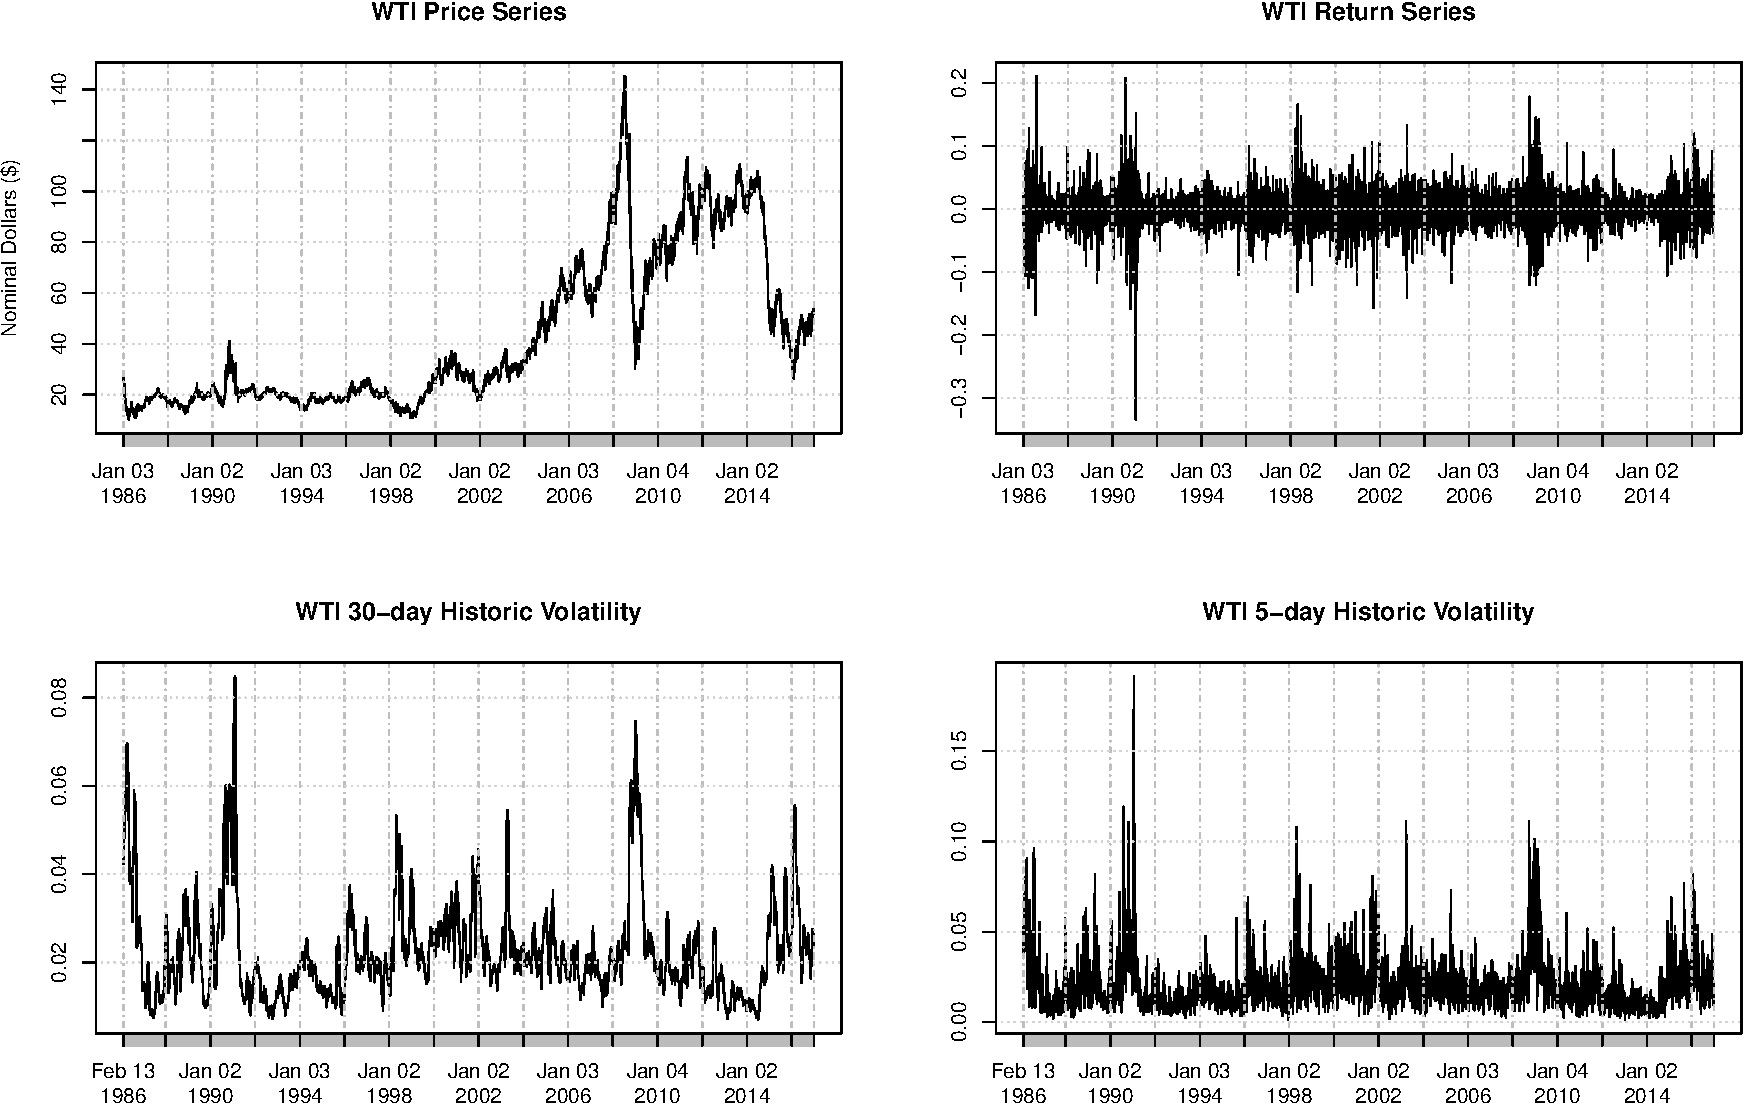
\includegraphics{Figs/unnamed-chunk-4-1.pdf}
\caption{Price level, return, and volatility series plots of WTI spot
oil prices.}
\end{figure}

\begin{figure}[htbp]
\centering
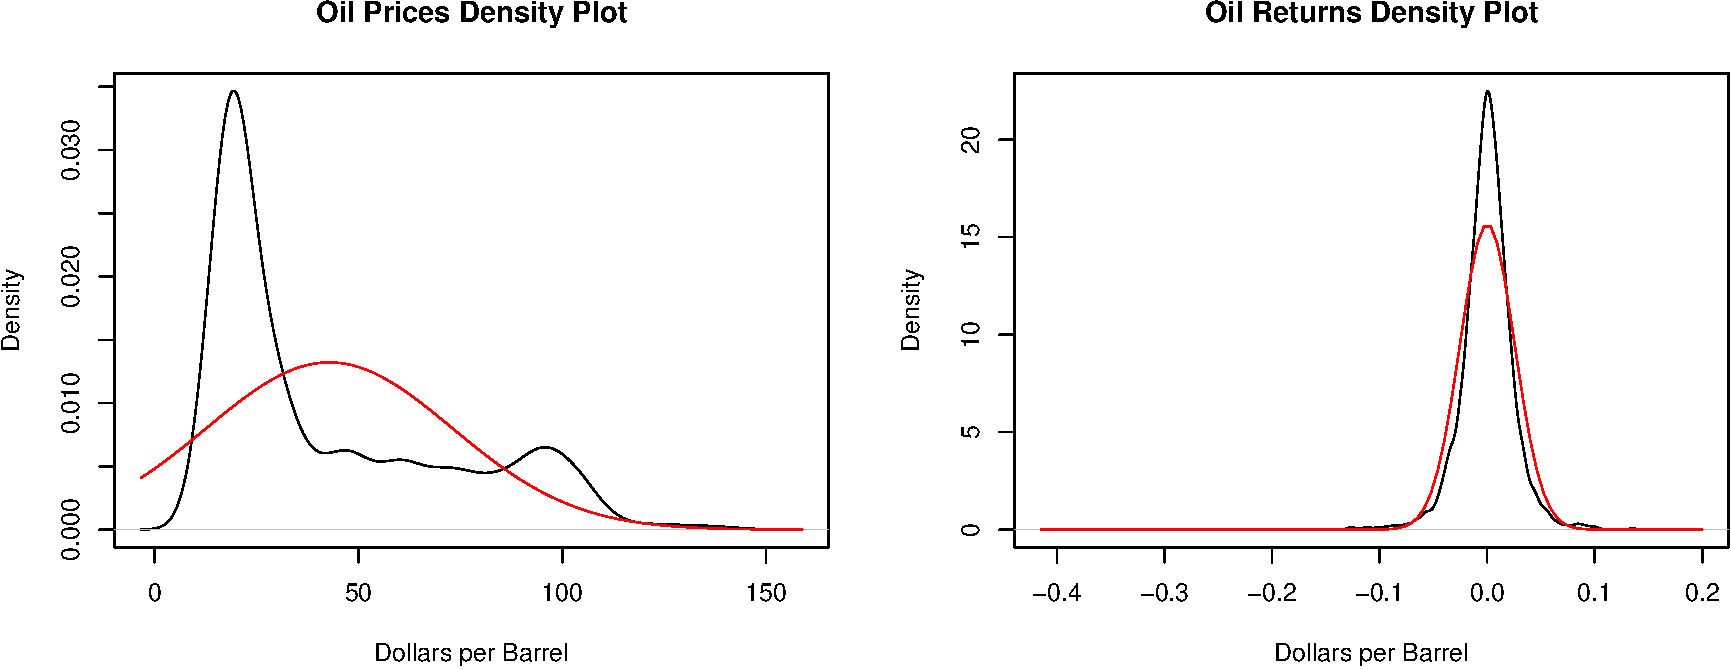
\includegraphics{Figs/unnamed-chunk-5-1.pdf}
\caption{Density plots demonstrating non-normality of price and return
series distributions.}
\end{figure}

\subsection{Times series exploration}\label{times-series-exploration}

A challenge in analyzing financial time series in general, and spot oil
market prices specifically, is that the variance structure may be
independent, but not identically distributed. Oil prices exhibit periods
of low volatility (i.e.~relatively constant prices) and periods of high
volatility (i.e.~changing prices). This is referred to as volatility
clustering. This violates the assumption in the most frequently used
time series model, the autoregressive integrated moving average (ARIMA)
model.

\begin{figure}[htbp]
\centering
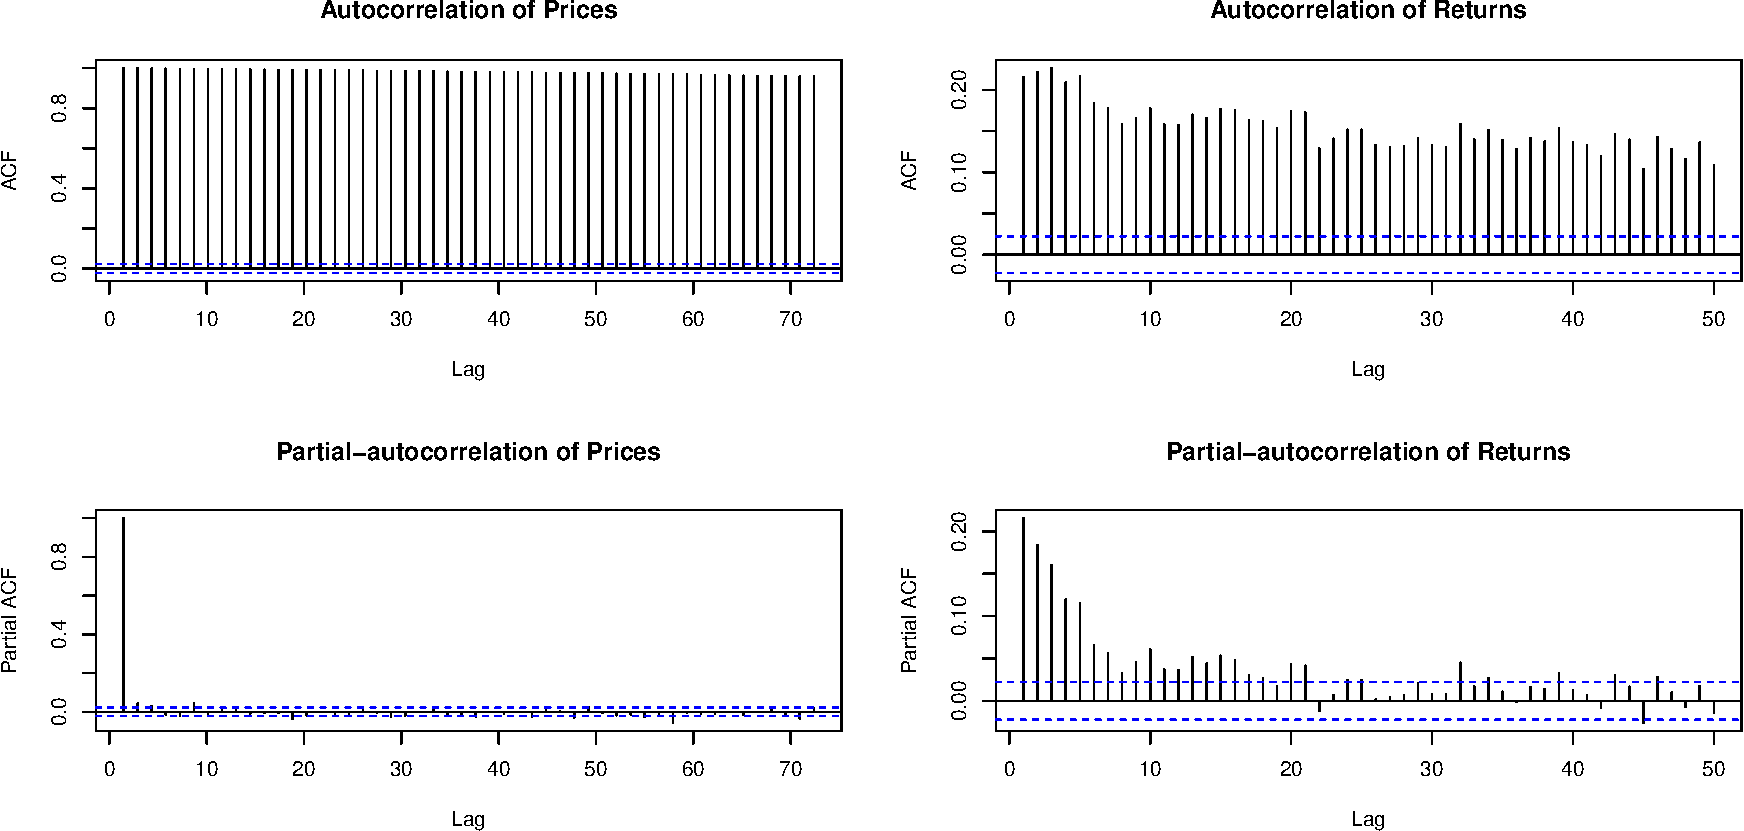
\includegraphics{Figs/unnamed-chunk-6-1.pdf}
\caption{Autocorrelation plots for prices and returns.}
\end{figure}

\section{Price-Volatility Regression
Analysis}\label{price-volatility-regression-analysis}

Relating price level and the measures of volatility at each time in the
series is a simple exploration of the research problem. The covariance
and correlation measures of vectors representing price versus returns,
30-day, and 5-day historic volatility indicate a weak, negative
relationship (Table 2).

\begin{longtable}[]{@{}lrr@{}}
\caption{Covariance and correlation of price level and returns, 30-day,
and 5-day historic volatility.}\tabularnewline
\toprule
& Covariance & Correlation\tabularnewline
\midrule
\endfirsthead
\toprule
& Covariance & Correlation\tabularnewline
\midrule
\endhead
return & -0.0396337 & -0.0719290\tabularnewline
30-day & -0.0640183 & -0.1864200\tabularnewline
5-day & -0.0529310 & -0.1212286\tabularnewline
\bottomrule
\end{longtable}

In quantitative finance, a process where volatility scales with price is
a lognormal process. When volatility is independent of price, the
process is normal (Ho and Lee, 2003). Regression of the price level and
squared returns is identified as the method of distinguishing lognormal
from normal processes in the literature. However, this simple method of
exploring the relationship between price level and volatlity does not
provide a satisfactory explanation. Volatility in financial time series
tend to cluster. Typically, some event (called a ``shock'') occurs which
results in an extremely high price movement. These are the large
noticable movements in the return series (Figure 1). Subsequent returns
are also of higher magnitude than the typical return size, but taper off
over time, eventually returning to a value close to the average return
for the price series.

\begin{figure}[htbp]
\centering
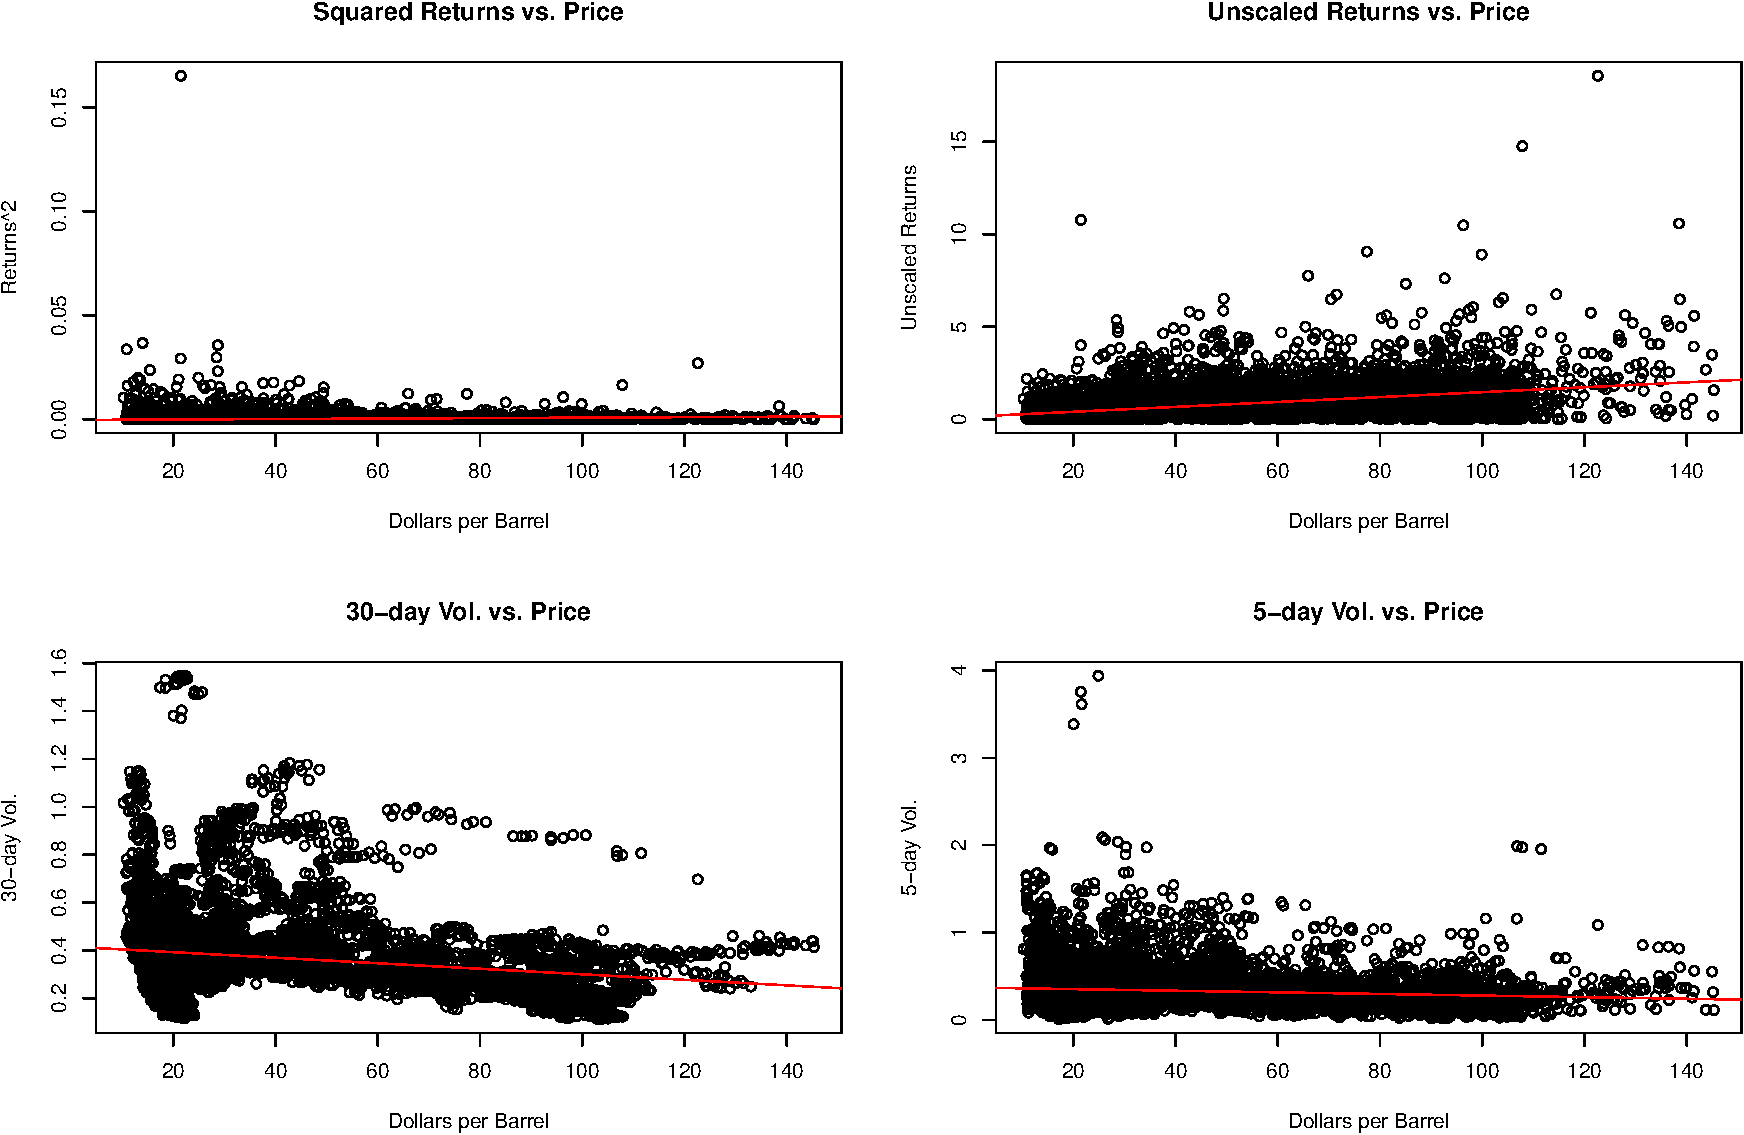
\includegraphics{Figs/unnamed-chunk-8-1.pdf}
\caption{Scatterplots with a linear model relating spot oil price with
returns, 30-day, and 5-day historic volatility.}
\end{figure}

The case of 30-day historic volatility indicates a negative relationship
between price level and volatility. However, this result appears to be
due to a cluster high volatility around \$20 per barrel, creating a
leverage point. Residual analysis indicates that this is not a good
relationship to model with linear regression. Residual analysis for the
other volatility measures also display

As seen in Figure 1, nominal oil prices have spent time as high as \$145
per barrel. However, the majority of the time series is far lower, with
a median price of \$28 per barrel. This means that the dataset is
unbalanced and higher price levels represent a smaller portion of the
dataset. In addition, oil price (and financial time series in general)
exhibits volatility clustering. Therefore, it is anticipated that this
simple regression model based on price and volatility is not the best
possible solution to the question of characterizing the dependency of
volatility on price. A second time series was created by limiting WTI
prices to the January 3, 1998 through December 31, 2016. This results in
a distribution that, while signficantly different than the normal
distribution, is more evenly distributed across the price range from
\$10.82 per barrel to \$145.30 per barrel (Figure 5). Given the ever
evolving economic, political, and technological landscape affect
commodity prices, there is some tradeoff between looking at a large
historic price record, which covers a larger data set of possible system
states (and higher statistical power), and limiting to a more recent
price record, which more fully represents the system in its current
state.\\
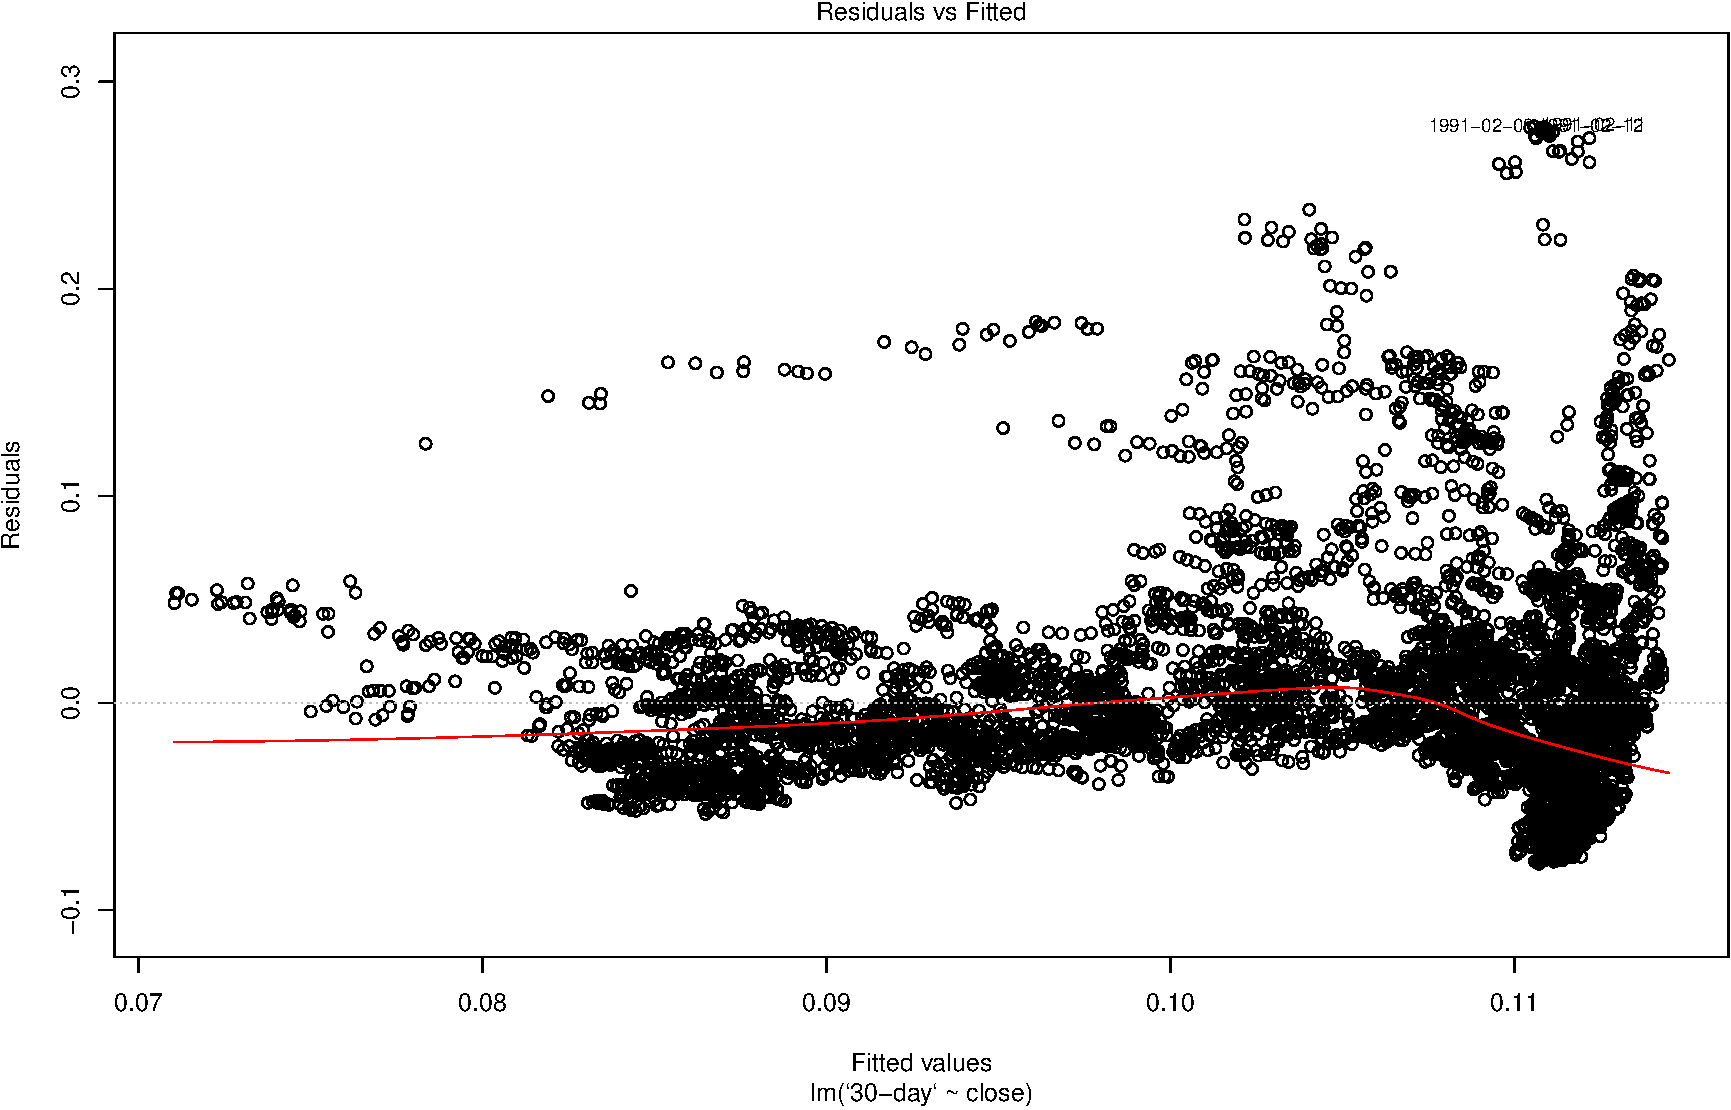
\includegraphics{Figs/unnamed-chunk-10-1.pdf}

\section{Comparing Volatility across Price
Regimes}\label{comparing-volatility-across-price-regimes}

In order to capture the volatility dynamics of the WTI price series,
including volatility clustering and changes in base price, it
changepoint detection was used to break the series into price regimes.
Changepoint detection aims to detect the point or points where the
statistical properties of a sequence of observations change (Killick and
Eckley, 2014). Changepoint detection was used to detect change in the
oil price mean throughout the period of record using the Pruned Exact
Linear Time (PELT) algorithm (Killick et al. 2012). The time series
between these changepoints represent ``price regimes'' (i.e.~time series
between changepoints) which have generally similar mean oil price
compared to the entire record.

Changepoint detection proceeds by minimizing a cost function over
possible locations and number of changepoints. The cost function:

\begin{figure}[htbp]
\centering
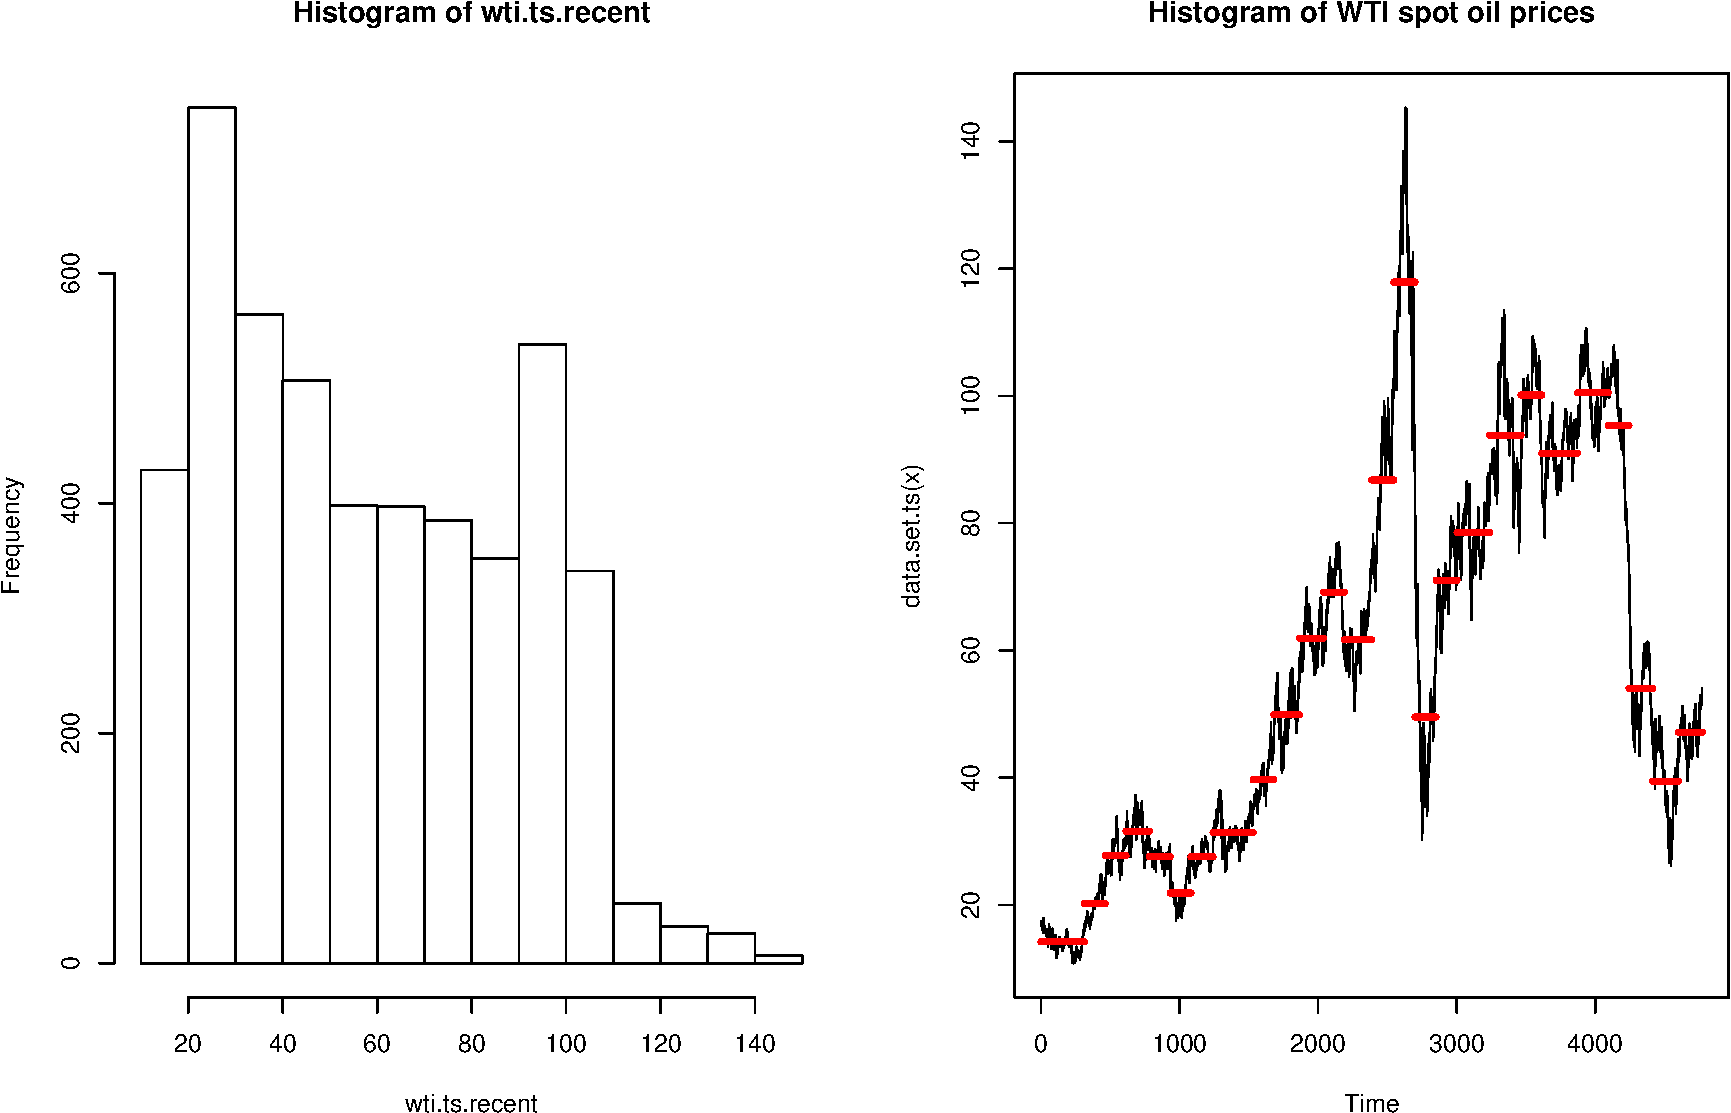
\includegraphics{Figs/unnamed-chunk-13-1.pdf}
\caption{Price regimes and linear model relating median oil price for
the regime to standard deviation within that price regime.}
\end{figure}

\begin{figure}[htbp]
\centering
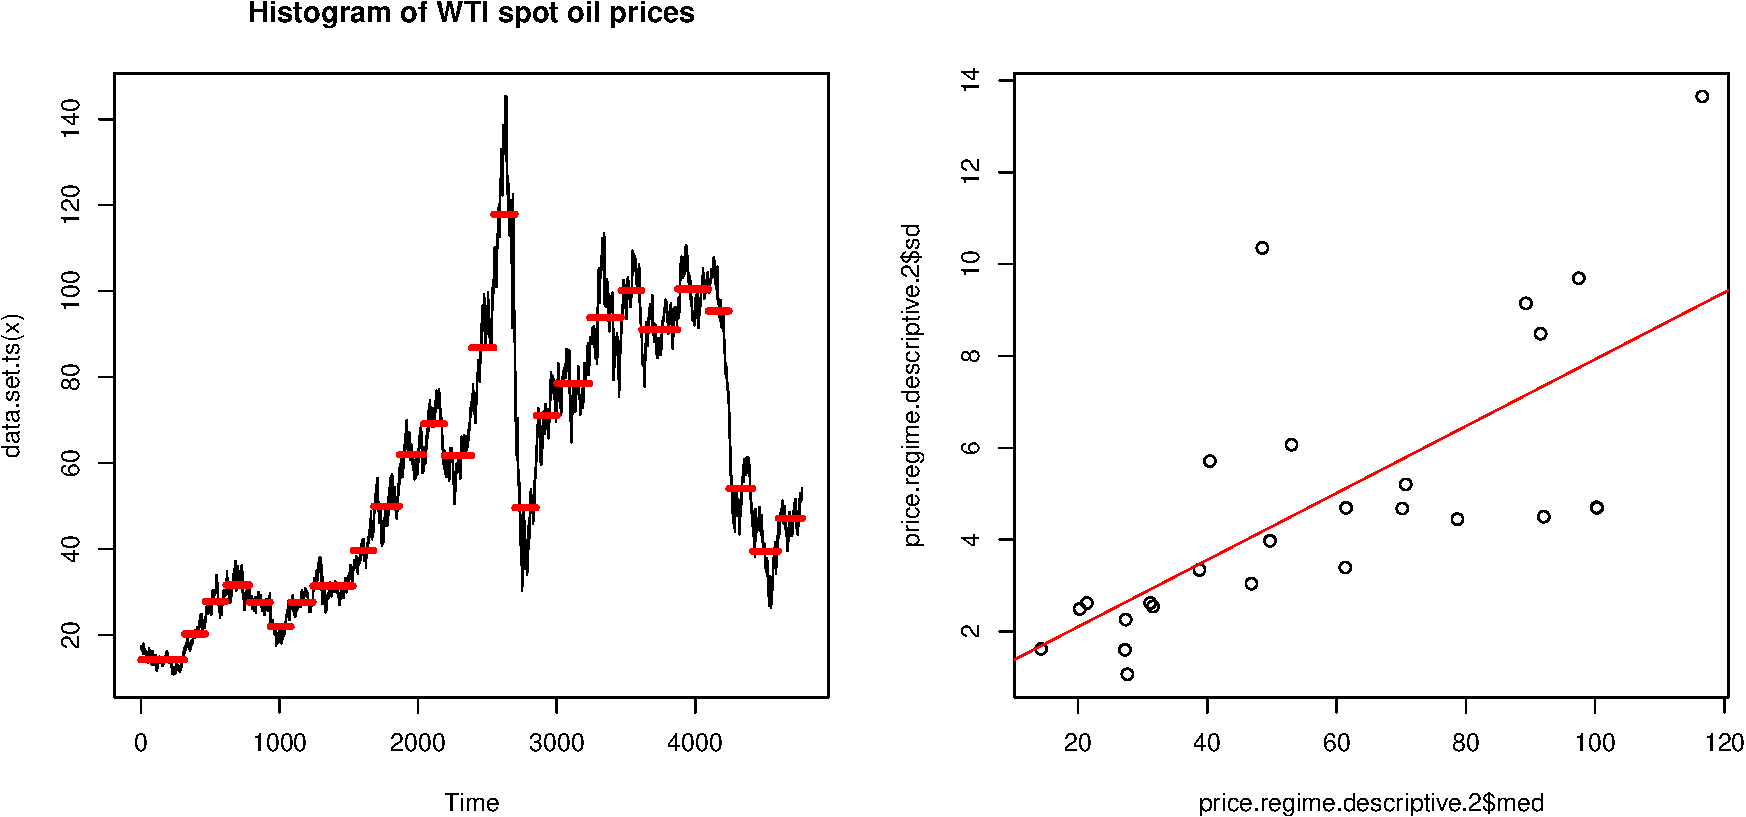
\includegraphics{Figs/unnamed-chunk-15-1.pdf}
\caption{Price regimes and linear model after limiting to 1998 through
2016.}
\end{figure}

This section's analysis using changepoint analysis to break the oil
price series into price regimes as defined by changes in the series mean
is highly dependent upon model parameters. The PELT changepoint
detection method identifies different changpoints depending on the
minimum segment length and penalty parameters, and based on the section
of the time series used. An interactive Shiny App was created and may be
access in order to try different parameterizations of the changepoint
model and view the effects on the relationship between medial regime
price and standard deviation within that regime.

\section{Multivariate GARCH Model}\label{multivariate-garch-model}

\section{Acknowledgements}\label{acknowledgements}

\emph{I would like to thank John Kemp, Thompson Reuters energy
journalist, for posing the question investigated in this research paper.
In addition, I thank Tancred Lidderdale and Mason Hamilton from the U.S.
Energy Information Administration for additional information pertaining
to the question.}

\section{Bibliography}\label{bibliography}

Thomas S. Y. Ho and Sang Bin Lee, 2004. The Oxford Guide to Financial
Modeling: Applications for Capital Markets, Corporate Finance, Risk
Management and Financial Institutions. ISBN: 9780195169621


\end{document}
